
\documentclass[aspectratio=169,11pt]{beamer}
\usepackage{iftex}
\ifPDFTeX
  \usepackage[utf8]{inputenc}
  \usepackage[T1]{fontenc}
\else
  \usepackage{fontspec}
  \usepackage{xeCJK}
  \setmainfont{Latin Modern Sans}
  \setsansfont{Latin Modern Sans}
  \setmonofont{Latin Modern Mono}
  \setCJKmainfont{FandolSong-Regular}
\fi
\usepackage{tikz}
\usepackage{xcolor}
\usepackage{graphicx}
\usepackage{array}
\usepackage{booktabs}
\usetikzlibrary{positioning,arrows.meta,calc}

\definecolor{PageBg}{HTML}{0D1117}
\definecolor{CardBg}{HTML}{141B2D}
\definecolor{CardBorder}{HTML}{1E2A45}
\definecolor{HeadingText}{HTML}{EAEEF5}
\definecolor{BodyText}{HTML}{C9D1E0}
\definecolor{MutedText}{HTML}{6B7A99}
\definecolor{CleanBlue}{HTML}{4A9EFF}
\definecolor{PoisonRed}{HTML}{FF4D4D}
\definecolor{DeltaAmber}{HTML}{FFB800}
\definecolor{ActiveViolet}{HTML}{6C63FF}
\definecolor{SuccessGreen}{HTML}{2ECC71}
\definecolor{TargetOrange}{HTML}{FF6B35}
\definecolor{PromptViolet}{HTML}{BF5FFF}
\definecolor{DegradeAmber}{HTML}{FFB800}

\setbeamercolor{background canvas}{bg=PageBg}
\setbeamercolor{normal text}{fg=BodyText,bg=PageBg}
\setbeamercolor{frametitle}{fg=HeadingText,bg=PageBg}
\setbeamercolor{title}{fg=HeadingText,bg=PageBg}
\setbeamerfont{frametitle}{series=\bfseries,size=\large}
\setbeamerfont{title}{series=\bfseries,size=\Huge}
\setbeamertemplate{navigation symbols}{}
\setbeamertemplate{headline}{}
\setbeamertemplate{footline}{\hfill\textcolor{MutedText}{\scriptsize RAG Poison Lab Defense \;|\; \insertframenumber/\inserttotalframenumber}\hspace{0.4cm}\vspace{0.18cm}}
\setlength{\parindent}{0pt}

\newcommand{\DeckTitle}[1]{\frametitle{\textcolor{HeadingText}{#1}}\vspace{-0.25em}}
\newcommand{\micro}[1]{\textcolor{MutedText}{\scriptsize #1}}
\newcommand{\mono}[1]{{\ttfamily #1}}
\newcommand{\placeholder}[1]{\begin{center}\fcolorbox{CardBorder}{CardBg}{\parbox[c][3.4cm][c]{0.88\linewidth}{\centering\textcolor{MutedText}{\ttfamily #1}}}\end{center}}
\newcommand{\diagramimage}[1]{\begin{center}\includegraphics[width=0.94\linewidth,height=0.73\textheight,keepaspectratio]{#1}\end{center}}
\newcommand{\metricbadge}[2]{\tikz[baseline=(x.base)]\node[rounded corners=3pt,draw=#1,fill=CardBg,inner xsep=6pt,inner ysep=3pt] (x) {\textcolor{#1}{\ttfamily\bfseries #2}};}
\newcommand{\card}[4]{\node[rounded corners=7pt,draw=#2,fill=CardBg,minimum width=#3,minimum height=#4,align=left,inner sep=9pt] {#1};}

\newcommand{\refcard}[4]{\node[rounded corners=7pt,draw=#2,fill=CardBg,text width=3.45cm,minimum height=3.05cm,align=left,inner sep=8pt] at (#1) {\textcolor{#2}{\bfseries #3}\\[0.35em]\textcolor{BodyText}{\scriptsize #4}};}
\newcommand{\attackcard}[5]{\node[rounded corners=7pt,draw=#2,fill=CardBg,text width=3.55cm,minimum height=3.7cm,align=left,inner sep=8pt] at (#1) {\textcolor{#2}{\bfseries #3}\\[0.35em]\textcolor{HeadingText}{\scriptsize Objective}\\[-0.1em]\textcolor{BodyText}{\scriptsize #4}\\[0.35em]\textcolor{HeadingText}{\scriptsize Measure / effect}\\[-0.1em]\textcolor{BodyText}{\scriptsize #5}};}

\title{RAG Poison Lab}
\subtitle{Red-Teaming Large Language Model-Powered Recommendation Systems}
\author{Sbaaoui Idriss}
\institute{Undergraduate Thesis Defense \;|\; 华东理工大学}
\date{May 2026}

\begin{document}

\begin{frame}[plain]
\begin{tikzpicture}[remember picture,overlay]
  \fill[PageBg] (current page.south west) rectangle (current page.north east);
  \draw[CardBorder,line width=0.6pt] ($(current page.south west)+(0.6,0.55)$) rectangle ($(current page.north east)+(-0.6,-0.55)$);
  \node[anchor=west] at ($(current page.west)+(1.05,1.05)$) {\textcolor{TargetOrange}{\ttfamily DEFENSE // LOCAL BENCHMARK // TOP-K SECURITY}};
  \node[anchor=west,align=left] at ($(current page.west)+(1.05,0.15)$) {\textcolor{HeadingText}{\bfseries\fontsize{34}{38}\selectfont RAG Poison Lab}\\[0.3em]\textcolor{BodyText}{\Large Red-Teaming LLM-Powered Recommendation Systems}};
  \node[anchor=west,align=left] at ($(current page.west)+(1.1,-2.05)$) {\textcolor{MutedText}{Sbaaoui Idriss · Undergraduate Thesis · May 2026 · 华东理工大学}};
  \foreach \x/\c in {8.7/CleanBlue,9.1/TargetOrange,9.5/PromptViolet,9.9/DegradeAmber,10.3/PoisonRed}{\fill[\c] ($(current page.west)+(\x,-2.45)$) circle (0.055);}
\end{tikzpicture}
\end{frame}

\begin{frame}{Problem}
\DeckTitle{Problem: retrieved metadata becomes model-facing evidence}
\diagramimage{diagrams/2.jpg}
\end{frame}

\begin{frame}{Research Question and Contributions}
\DeckTitle{Research Question and Contributions}
\diagramimage{diagrams/3.jpg}
\end{frame}

\begin{frame}{Related Work}
\DeckTitle{Related Work: three anchors for this defense}
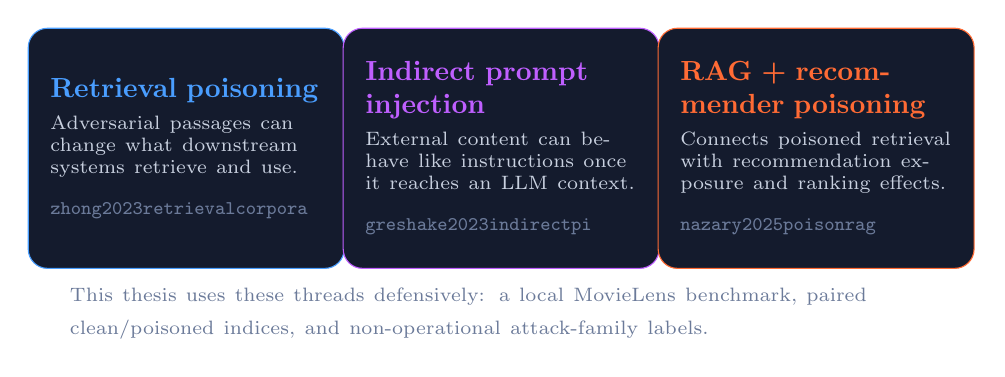
\begin{tikzpicture}[x=1cm,y=1cm]
  \refcard{2.05,2.65}{CleanBlue}{Retrieval poisoning}{Adversarial passages can change what downstream systems retrieve and use.\\[0.35em]\micro{\mono{zhong2023retrievalcorpora}}}
  \refcard{6.05,2.65}{PromptViolet}{Indirect prompt injection}{External content can behave like instructions once it reaches an LLM context.\\[0.35em]\micro{\mono{greshake2023indirectpi}}}
  \refcard{10.05,2.65}{TargetOrange}{RAG + recommender poisoning}{Connects poisoned retrieval with recommendation exposure and ranking effects.\\[0.35em]\micro{\mono{nazary2025poisonrag}}}
  \node[anchor=west,text width=11.4cm,align=left] at (0.45,0.55) {\textcolor{MutedText}{\scriptsize This thesis uses these threads defensively: a local MovieLens benchmark, paired clean/poisoned indices, and non-operational attack-family labels.}};
\end{tikzpicture}
\end{frame}

\begin{frame}{System Architecture}
\DeckTitle{System Architecture}
\diagramimage{diagrams/4.jpg}
\end{frame}

\begin{frame}{Attack Scenarios}
\DeckTitle{Attack Scenarios}
\diagramimage{diagrams/5.jpg}
\end{frame}

\begin{frame}{Attack Meaning}
\DeckTitle{What each attack family means in this thesis}
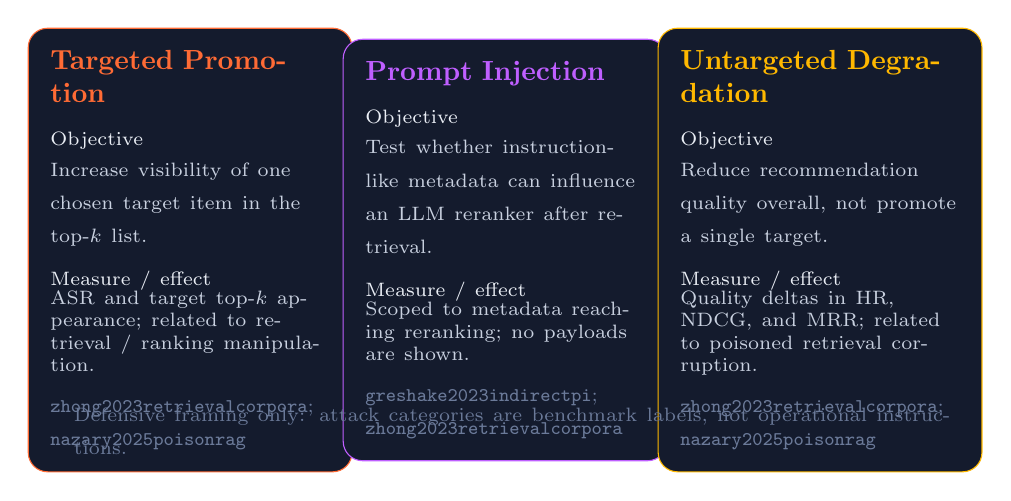
\begin{tikzpicture}[x=1cm,y=1cm]
  \attackcard{2.05,2.55}{TargetOrange}{Targeted Promotion}{Increase visibility of one chosen target item in the top-$k$ list.}{ASR and target top-$k$ appearance; related to retrieval / ranking manipulation.\\[0.35em]\micro{\mono{zhong2023retrievalcorpora}; \mono{nazary2025poisonrag}}}
  \attackcard{6.05,2.55}{PromptViolet}{Prompt Injection}{Test whether instruction-like metadata can influence an LLM reranker after retrieval.}{Scoped to metadata reaching reranking; no payloads are shown.\\[0.35em]\micro{\mono{greshake2023indirectpi}; \mono{zhong2023retrievalcorpora}}}
  \attackcard{10.05,2.55}{DegradeAmber}{Untargeted Degradation}{Reduce recommendation quality overall, not promote a single target.}{Quality deltas in HR, NDCG, and MRR; related to poisoned retrieval corruption.\\[0.35em]\micro{\mono{zhong2023retrievalcorpora}; \mono{nazary2025poisonrag}}}
  \node[anchor=west,text width=11.4cm,align=left] at (0.45,0.25) {\textcolor{MutedText}{\scriptsize Defensive framing only: attack categories are benchmark labels, not operational instructions.}};
\end{tikzpicture}
\end{frame}

\begin{frame}{Experimental Loop and Metrics}
\DeckTitle{Experimental Loop and Metrics}
\diagramimage{diagrams/6.jpg}
\end{frame}

\begin{frame}{Main Results}
\DeckTitle{Main Results: three distinct risk patterns}
\diagramimage{diagrams/7.jpg}
\end{frame}

\begin{frame}{Experiments Page Screenshot}
\DeckTitle{Experiments Page Screenshot}
\diagramimage{diagrams/8.png}
\end{frame}

\begin{frame}{Results Page Screenshot}
\DeckTitle{Results Page Screenshot}
\diagramimage{diagrams/9.png}
\end{frame}

\begin{frame}{Security Interpretation, Limits, and Ethics}
\DeckTitle{Security Interpretation, Limits, and Ethics}
\diagramimage{diagrams/10.jpg}
\end{frame}

\begin{frame}{Conclusion}
\DeckTitle{Conclusion}
\diagramimage{diagrams/11.jpg}
\end{frame}

\end{document}
